\documentclass[a4paper, 12 pt]{article}
\usepackage[utf8]{inputenc}
\usepackage[T1]{fontenc}
\usepackage[slovene]{babel}
\usepackage{lmodern}
\usepackage{amsmath}
\usepackage{amsfonts}
\usepackage{amssymb}
\usepackage{units}
\usepackage{eurosym}
\usepackage{pdfpages}
\usepackage{comment}
\usepackage{enumerate}
\usepackage{mathtools}
\usepackage{amsthm}
\usepackage{float}


% ukazi za matematicna okolja
\theoremstyle{definition} % tekst napisan pokoncno
\newtheorem{definicija}{Definicija}[section]
\newtheorem{primer}[definicija]{Primer}
\newtheorem{opomba}[definicija]{Opomba}

\renewcommand\endprimer{\hfill$\diamondsuit$}


\theoremstyle{plain} % tekst napisan posevno
\newtheorem{lema}[definicija]{Lema}
\newtheorem{izrek}[definicija]{Izrek}
\newtheorem{trditev}[definicija]{Trditev}
\newtheorem{posledica}[definicija]{Posledica}
\theoremstyle{definition}
\newtheorem{definition}{Definicija}[section]




% za stevilske mnozice uporabi naslednje simbole
\newcommand{\R}{\mathbb R}
\newcommand{\N}{\mathbb N}
\newcommand{\Z}{\mathbb Z}
\newcommand{\C}{\mathbb C}
\newcommand{\Q}{\mathbb Q}

% ukaz za slovarsko geslo
\newlength{\odstavek}
\setlength{\odstavek}{\parindent}
\newcommand{\geslo}[2]{\noindent\textbf{#1}\hspace*{3mm}\hangindent=\parindent\hangafter=1 #2}

% naslednje ukaze ustrezno popravi
\newcommand{\program}{Finančna matematika} % ime studijskega programa: Matematika/Finan"cna matematika
\newcommand{\imeavtorja}{Sabrina Calcina in Jan Črne} % ime avtorja
\newcommand{\imementorja}{prof. dr. Sergio Cabello in asist. dr. Janoš Vidali} % akademski naziv in ime mentorja
\newcommand{\naslovdela}{Algoritmi in množice neodvisnosti za podatkovno vodene robustne probleme najkrajših poti}
\newcommand{\letnica}{2020} %letnica diplome
\newcommand{\norm}[1]{\left\lVert#1\right\rVert}







\begin{document}

\thispagestyle{empty}
\noindent{\large
UNIVERZA V LJUBLJANI\\[1mm]
FAKULTETA ZA MATEMATIKO IN FIZIKO\\[5mm]
\program\ -- 1.~stopnja}
\vfill

\begin{center}{\large
\imeavtorja\\[2mm]
{\bf \naslovdela}\\[10mm]
Finančni praktikum\\[1cm]
Mentor: \imementorja}
\end{center}
\vfill

\noindent{\large
Ljubljana, \letnica}
\pagebreak

\thispagestyle{empty}
\tableofcontents
\pagebreak


\thispagestyle{empty}
\begin{center}
{\bf \naslovdela}\\[3mm]
{\sc Povzetek}
\end{center}
V prejktu smo se ukvarjali z  robustnimi problemi najkrajših poti. To so problemi, katerih cilj je najti pot, ki optimizira najslabše delovanje v množici negotovosti. Množica negotovosti je množica, ki vsebuje vse scenarije cen povezav, zgeneriranih ali zabeleženih na podlagi opažanj.
Predpostavka tega problema je, da so množice negotovosti podane s strani strokovnjakov, ki povedo obliko in velikost le te.
Množice negotovosti smo v projektu naključno generirali. Meriteve uporabljene v članku, na katerem sloni najino delo, temeljijo na resničnih podatkih iz meritev prometa. Na podlagi teh podatkov, ki torej vsebujejo cene povezav nekega usmerjenega grafa, nato po premisleku izberemo primerno množico negotovosti, tako da primerjamo uspešnost dobljenih robustnih poti. 
Na podlagi že znanih eksperimentov o učinkovitosti elipsoidne negotovosti, se nato osredotočimo na elipsoidne množice negotovosti na katerih preiskušamo dva algoritma  za iskanje najcenejše povezave med začetnim in končnim vozliščem.
\vfill


\pagebreak

\section{Uvod}
Za klasične probleme najkrajših poti v uličnih omrežjih so bile dosežene znatne pospešitve v primerjavi s standardnim Dijkstrovim algoritmom. Zahvala gre tehnikam novejših algoritmov, ki omogočajo uporabo informacij v realnem času, tudi v velikih omrežjih.
Kljub temu je večina robustnih problemov z najkrajšimi oz. najcenejšimi potmi časovno zahtevna in optimizacija v realnem času ni na voljo. Za oblikovanje robustnega problema je tako treba imeti opis vseh možnih in ustreznih scenarijev, na katere naj bi se pripravili.\newline

Prvi članek, ki sledi drugačni perspektivi problema najkrajše poti, je izšel leta 2017. Gre za robustno optimizacijo, ki temelji na podatkih, kjer je gradnja negotove množice na podlagi surovih opazovanj del robustnega problema optimizacije. Na podlagi realnih opazovanj mesta Chicago so tako izračunali ustrezne robustne rešitve in izvedli poglobljeno analizo njihove uspešnosti. \newline

V delu se osredotočimo na primer elipsoidne negotovosti za katero preiskušamo algoritme. 


\section{Opis problema}
\begin{itemize}
\item{Za začetek imamo usmerjen graf $ G = (V, A)$, kjer je $V$ je množica vozljev, ter $A$ množica povezav. Za vsako povezavo je znana njena cena, ki bo v našem primeru čas, potreben za prehod te povezave.}
\item{Cilj je najti pot v grafu, ki minimizira čas potreben za pot od začetnega do končnega vozlišča. Za razliko od nam do zdaj znanih primerov, kjer so bile cene povezav podane eksaktno, so v našem primeru te podane z množico opazovanj teh povezav.}
\item{Na teh množicah lahko sedaj poiščemo takšno pot, da bomo zminimizirali časovno najugodnejšo pot v primeru najslabšega scenarija. Npr. želimo poiskati najkrajšo pot v mestu od ene točke do druge, v primeru, maksimalne zasedenosti cest. Torej takrat, ko za vožnjo po njih porebujemo največ časa.}
\item{Osredotočili se bomo na izvajanje algoritma za iskanje teh poti na elipsoidinih množicah negotovosti. Le te ponudijo najbolše razmerje med maksimalno in povprečno potjo, ter ponudijo zadovoljivo časovno zahtevnost algoritma.}
\item{Prvotno smo tako izvedli Naivni algoritem, kasneje pa še Izboljšanega.}
\end{itemize}


\section{Množice negotovosti najkrajših poti}

Naj bo $G = (V, A)$ graf, kjer z $V$ označimo vozlišča grafa in z $A$ poti. Za vsako pot $e\in A$ poznamo čas potovanja $c_{e} \ge 0$. Začetno vozlišče označimo s $s$, končno pa s $t$.
Cilj je najti najkrajšo pot, ki minimizira celoten čas potovanja, podan kot vsoto vseh časov na določeni povezavi, ki je del poti. Formalno to zapišemo kot

\begin{equation*}
\min \{c^t x : x \in \chi \},
\end{equation*}

kjer je $\chi \subseteq \{0,1\}^n$ in $n = |A|$.\newline

Predpostavimo tudi, da čas potovanja ni natančno znan, vendar je le ta podan kot množica $R$, kjer je $R = \{c^1, \dots, c^N \}$.\newline

Na podlagi teh podatkov generiramo množice negotovosti $U$, ki jih uporabljamo pri robustnih problemih najkrajših poti

\begin{equation*}
\min \{\max \limits_{c \in U} c^t x : x \in \chi \}.
\end{equation*}
 Torej iščemo pot, ki minimizira najslabše možnosti cen, glede na vse cene v $U$.

\bigskip

Naj bo sedaj $\hat{c} = \frac{1}{N} * \sum_{i \in [N]} c^i $, kjer je $[N] = \{1, \dots , N \}$. Elipsoidno negotovost za parameter $\lambda$ definiramo kot
\begin{equation*}
U^E = \{c: (c - \hat{c})^t \Sigma ^{-1} (c - \hat{c}	\le \lambda \},
\end{equation*}

kjer je $\Sigma = \frac{1}{N} \sum_{i \in [N]} (c^i -\hat{c}) (c^i -\hat{c})^t$.

\bigskip
Poleg elipsoidne negotovosti, poznamo tudi negotovost konveksnega trupa, intervalsko negotovost ter negotovost permotohula in druge. 
\pagebreak


\section{Priprava}

Najprej smo generirali množice negotovosti velikosti $50$, torej za vsako povezavo v grafu je bilo danih $50$ različnih cen oziroma opažanj. Cene so porazdeljene enakomerno, vrednosti so iz množice od $\{1, \dots , 100\} $. Vsaki povezavi smo nato naračunali povprečno ceno, povprečja vseh teh povezav so zbrana v vektorju $\hat{c}$.\newline


\begin{figure}[H]
    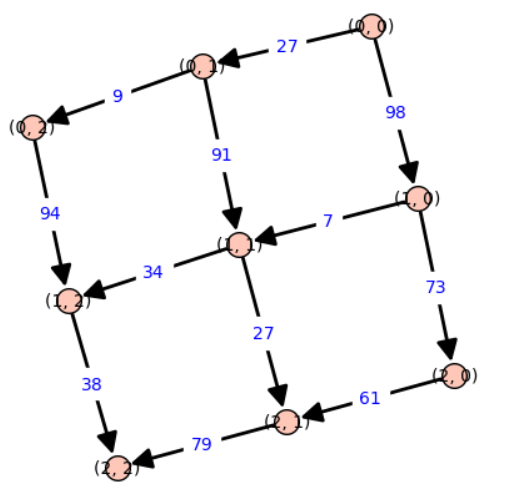
\includegraphics[width=.5\textwidth]{prvi.png}\hfill
    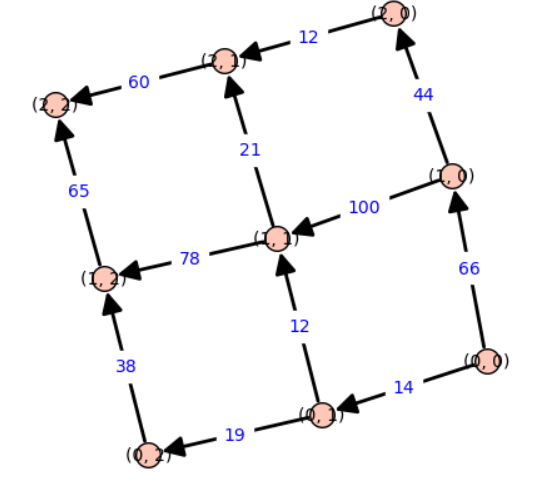
\includegraphics[width=.5\textwidth]{drugi.png}\hfill
    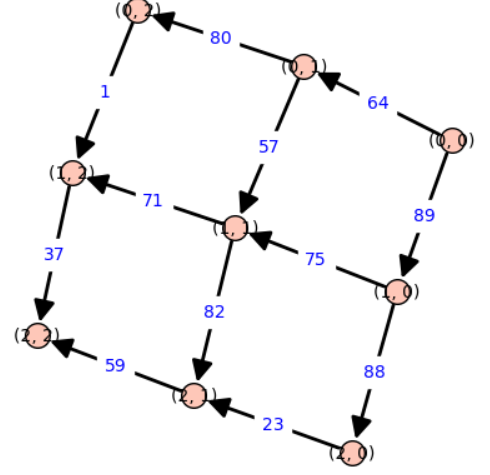
\includegraphics[width=.5\textwidth]{tretji.png}\hfill
    \\[\smallskipamount]
    \caption{Prikaz na mrežatih grafih velikosti $3 \times 3$ za tri opažanja}\label{fig:foobar}
\end{figure}

  
V nalogi smo obravnavali dva algoritma , ki iščeta najcenejšo robustno rešitev. Algoritma smo prizkušali na usmerjenih mrežasti grafih, v našem primeru na grafih  z od $3\times3$, do $9\times9$ vozliščih. Za vsakega od teh grafov smo iskali pot od začetnega vozlišča $(1, 1)$ do skrajno robnega vozlišča s koordinatami $(V, V)$. Za potrebo algoritmov, smo morali najti vse možne poti med tema dvema vozliščema, če je poti med vozliščema $p$, smo potem priredili vektorje iz množice $X = \{x^1, \dots, x^p \}$, vektorji so sestavljeni iz elementov $1$, v kolikor je povezava v poti uporabljena in $0$, če je izpuščena. Velja omeniti še, da je število povezav mrežastih grafov in število poti med skrajnima vozliščema neposredno odvisno števila vozlišč grafa.\newline

Pred pričetkom uporabe algoritmov smo pridobili še diagonalne elemente matrike $\Sigma$, ki je naračunana iz množic negotovosti, torej predstavlja elipsoidono množico negotovosti.


\section{Predstavitev optimizacijskega problema elipsoidnih množic negotovosti}
Ker so elipsoidne množice negotovosti zelo stabilne in splošno zelo učinokovite, glede na ostale navedene negotovosti, smo se osredotočili na le te.

Sprva opišimo učinkovit algoritem za reševanje problema robustne najkrajše poti, če je množica negotovosti podana kot osem paralelni elipsoid. Formulacija tega problema je

\begin{equation*}
\begin{aligned}
\min \quad &  \hat{c}^t x + z\\
\textrm{p.p.} \quad & {z}^2 \geq (x^t \Sigma x )\\
& x \in \chi,\\
\end{aligned}
\end{equation*}
 kjer $\Sigma$ predstavlja diagonalo matrike, ki specificira obliko in velikost elipsoida. \newline

Naj bo $d$ diagonala matrike $\Sigma$.
Ker velja, da je $x$ binaren vektor in s tem $x_{i}^2=x_{i}$, poleg tega pa velja, da je $(x^t  \Sigma x)^2 = d^tx$, lahko problem zreduciramo na

\begin{equation*}
\begin{aligned}
\min \quad &  \hat{c}^t x +\sqrt{d^tx}\\
\textrm{p.p.} \quad & x \in \chi.\\
\end{aligned}
\end{equation*}

Problem lahko transformiramo na bikriterijski optimizacijski problem, podan kot

\begin{equation*}
\begin{aligned}
\min \quad &  \begin{pmatrix} \hat{c}^t x \\ d^tx \end{pmatrix} \\
\textrm{p.p.} \quad & x \in \chi.\\
\end{aligned}
\end{equation*}

Rešitev robustnega problema je v resnici tudi rešitev bikriterijskega optimizacijskega problema. Rešitvi zgornjega problema $x^*$ rečemo $učinkoviti\;ekstrem$, če obstajata  $\alpha_{0}$ in $\alpha_{1}$, velja $0 \le \alpha_{0} < \alpha_{1} \le 1$. Tako da za vse $\alpha \in [\alpha_{0},\alpha_{1}]$  ne obstaja neka druga rešitev $x'$, za katero bi veljalo $(\alpha c + (1 - \alpha)d)^tx' < (\alpha c + (1- \alpha)d)^tx^{*}$.\newline
 To pomeni, da je dovolj, če rešimo naslednji problem
\begin{equation*}
\begin{aligned}
\min \quad &  \alpha c + (1 - \alpha)d)^tx \\
\textrm{p.p.} \quad & x \in \chi.\\
\end{aligned}
\end{equation*}

Ker je rešitev lahko precej zahtevna, se omejimo na računanje podmnožic vseh učinkovitih ekstremnih rešitev problema. Med najdenimi rešitvami se nato izbere najboljša glede na robustno ciljno funkcijo.\newline


Oba algoritma iščeta učinkovite oz. učinkovito ekstremno rešitev s pomočjo računanja optimizacije leksikografskega problema
\begin{equation*}
\begin{aligned}
\text{arglexmin}\quad &  (\hat{c}^t x , {d^tx})\\
\textrm{p.p.} \quad & x \in \chi.\\
\end{aligned}
\end{equation*}

pri obeh je potrebno naračunati $x_l$ in $x_r$, kjer eden minimizira skalarni produkt po $\hat{c}$, drugi pa po $d$, eden torej poišče najcenejšo pot po povprečjih povezav, drugi pa po diagonalnih vrednostih matrike.\newline

Naivni algoritem učinkovite ekstremne rešitve išče rekurzivno, tako da vedno znova poišče najcenejšo pot, jo nato primerja z prejšnjo najcenejšo potjo in v kolikor pride do izbolšave doda v množico ekstremnih rešitev novo vrednost.

Izboljšani algoritem, pa se s pomočjo $x_l$ in $x_r$ omeji na neko območje iskanja rešitev, območje iskanja z vsako novo najdeno izboljšano rešitvijo zmanjša, ko je območja iskanja prazno ali zadosti majhno pa se algoritem ustavi ter vrne najugodnejšo pot.


\section{Naivni algorotem in njegovi rezultati}

Na začetku dela, smo se reševanja problema lotili z uporabo naivnega algoritma. Ko smo naivni algoritem pognali na mrežnih grafih, je le ta vrnil množico učinkovitih ekstremnih rešitev, torej poti, katere dokaj dobro rešijo robustni problem najcenejših poti. Poleg tega, naju je zanimala še časovna zahtevnost algoritma in kolikokrat se je znotraj algoritma reševal problem najkrajših poti.
Za vsak mrežast graf z $n \times n$ vozlišči, smo naredili 30 ponovitev, ter izračunali povprečno vrednost poganjanja. Rezultate smo za $n = 3, 4, 5, 6, 7, 8, 9$ predstavili v spodnji tabeli.\newline


Naj bo Graf n, graf z $n \times n$ vozlišči, čas je podan v sekundah.

\begin{center}
 \begin{tabular}{||c c c c c c c||} 
 \hline
Graf 3 & Graf 4 & Graf 5 & Graf 6 & Graf 7 & Graf 8 & Graf 9 \\ 
 \hline
\hline
0.00078 & 0.00533 & 0.02949 & 0.24377 & 1.17852 & 7.36974 & 40.05113 \\
 \hline
\end{tabular}
\end{center}

Komputacijski čas je vračal pričakovane vrednosti in sicer, za grafe z večjimi vozlišči je potreboval več časa. Za grafe z $9 \times 9$ vozlišči je potreboval nekaj več kot 40 sekund, medtem ko je manjše grafe algoritem predelal zelo hitro. Komputacijski čas bomo kasneje primerjali z komputacijskim časom izboljšanega algoritma.\newline

Poleg tega, smo beležili tudi kolikokrat je za posamezno velikost grafa algoritem reševal problem najkrajših poti. Število reševanj je predstavljeno v spodnji tabeli.\newline

\bigskip
Naj bo NP n, število ki nam pove, koliko krat je algoritem pregledal celotno množico x, za katero je potem našel najkrajšo možno pot glede na dan optimizacijski problem za grafe z $n \times n$ vozlišči.
\begin{center}
 \begin{tabular}{||c c c c c c c||} 
 \hline
 NP 3 &  NP 4 &  NP 5 &  NP 6 &  NP 7 &  NP 8 &  NP 9 \\ 
 \hline
\hline
2.07 & 2.47 & 4.07 & 5.73 & 6.53 & 8.2 & 8.93\\
 \hline
\end{tabular}
\end{center}


Za večje grafe je algoritem večkrat reševal problem, kar je torej podaljšalo komputacijski čas. Tudi rekurzivne klice bomo kasneje primerjali z izboljšanim algoritmom.


\section{Izboljšani algoritem in njegovi rezultati}

Na enakih grafih kot pri naivnem algoritmu, torej mrežastih, smo poskus ponovili na izboljšanem algoritmu. Naredili smo 30 ponovitev, ter izračunali povrpečno vrednost poganjanja. Rezultate za $ n = 3,4,5,6,7,8,9$ smo predstavili v spodnji tabeli.


Naj bo Graf n, graf z $n \times n$ vozlišči, komputacijski čas je podan v sekundah.
\begin{center}
 \begin{tabular}{||c c c c c c c||} 
 \hline
Graf 3 & Graf 4 & Graf 5 & Graf 6 & Graf 7 & Graf 8 & Graf 9 \\ 
 \hline
\hline
0.11760 & 0.01872 & 0.02816 & 0.16980 & 0.64850 & 2.38989 & 17.06119\\
 \hline
\end{tabular}
\end{center}

Tudi izboljšani algoritem je, pričakovano za večje grafe z več potmi, v povprečju potreboval dalj časa.\newline


Poleg tega, smo ponovno beležili kolikokrat je za posamezno velikost grafa algoritem reševal problem najkrajših poti. Število reševanj je predstavljeno v spodnji tabeli.


Naj bo NP n enako kot zgoraj, le da tokrat torej uporabljamo izboljšani algoritem. 
\begin{center}
 \begin{tabular}{||c c c c c c c||} 
 \hline
 NP 3 &  NP 4 &  NP 5 &  NP 6 &  NP 7 &  NP 8 &  NP 9 \\ 
 \hline
\hline
3.87 & 4.07 & 3.20 & 4.00 & 4.27 & 3.47 & 4.6 \\ 
 \hline
\end{tabular}
\end{center}

Izboljšani algoritem, zanimivo problema najkrajših poti ne računa nujno večkrat za grafe z več vozlišči, kar pomeni, da kot kaže, s svojimi pogoji že v prvih korakih določi dokaj dober približek najugodnejše poti za robusten optimizacijski problem. 

\section{Primerjava algoritmov}

Opažanja smo predstavili na spodnjem grafu. 

\begin{figure}[H]
  \centering
  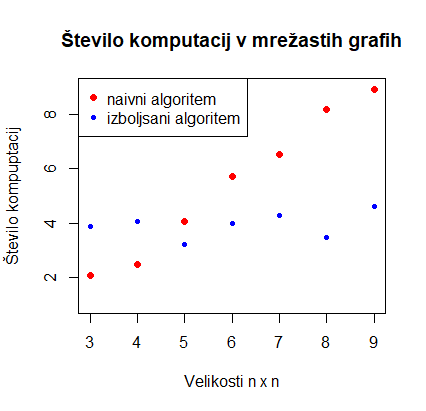
\includegraphics[width=90mm]{Rplot2.png}
  \caption{Število komutacijskih časov v mrežastih grafih}
  \label{fig: Graf 1}
\end{figure}

Razvidno je, da števila komputacij pri naivnem algoritmu naraščajo bistveno hitreje kot kot pri izboljšanem, kjer povečave skoraj ni bilo. Število komputacij pri 30 ponovitvah $9 \dots 9$ grafov, je tako število komputacij v povprečju nekaj več kot 4, pri naivnem pa skoraj 9.\newline

Komputacijske čase obeh algoritmov smo predstavili na spodnjem grafu.

\begin{figure}[H]
  \centering
  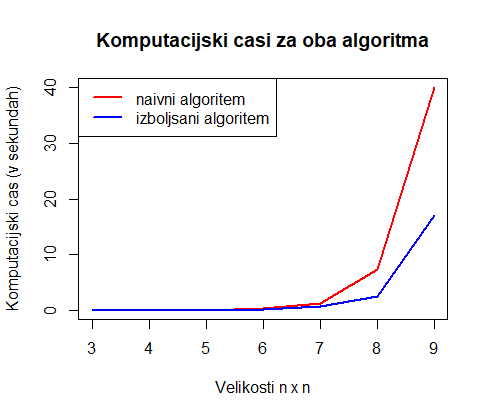
\includegraphics[width=90mm]{Rplot3.png}
  \caption{Število komutacijskih časov v mrežastih grafih}
  \label{fig: Graf 1}
\end{figure}


Razvidno je, da izboljšani algoritem poti išče mnogo hitreje kot naivni. V iskanju robustnih rešitev, je časovno najzahtevnejše iskanje najkrajših poti. Izboljšani algoritem problem rešuje manjkrat, tako je pri istem številu vozlišč časovna zahtevnost nižja.

\newpage


\begin{thebibliography}{9}

    \bibitem{RNP} 
    André Chassein, Trivikram Dokka, Marc Goerigk
    \\\texttt{Algorithms and uncertainty sets for data-driven robust shortest path problems}

\end{thebibliography}



















\end{document}